\hypertarget{denavit-hartenberg-convention}{%
\section{\texorpdfstring{\texttt{Denavit-Hartenberg\ Convention}}{Denavit-Hartenberg Convention}}\label{denavit-hartenberg-convention}}

In a number of science fiction movies you will see (CGI) versions of
serial chain manipulators that have a large number of links. These
manipulator twist around in space and do some amazing things. We also
know that movie evil geniuses are smart - hence the name evil genius.
However, we know that most are rather impatient. How, you wonder did
they stick with all of the algebra to compute forward and inverse
kinematics. The answer is that they also had a "tabular" or automated
approach to the problem. This is what we introduce in this section - a
convention for systematically computing the forward kinematics.

Given joint angles and actuator lengths one can compute the end effector
position. Thus it is possible to compute the effector path as a function
of arm movements.

\[\begin{pmatrix} \theta_1(t), ... , \theta_n(t)
           \end{pmatrix}\to p(t)\]

A simple way to relate the end effector to the base for a serial chain
manipulator is to see each link as a transformation of the base
coordinate system. This is the approach suggested by Denavit and
Hartenberg.

\hypertarget{denavit-hartenberg-parameters}{%
\subsection{\texorpdfstring{\texttt{Denavit-Hartenberg\ Parameters}}{Denavit-Hartenberg Parameters}}\label{denavit-hartenberg-parameters}}

The DH convention provides a standard way to build kinematic models for
a robot. It is a simple concept and the complexity is hidden in the
composition of linear transformations. This provides a powerful way to
generate the kinematic equations in a consistent form. As suggested
above, we follow out the links of the manipulator, and see them as
rotations and translations of the coordinate system:

\begin{quote}
\[A = A_0 A_1 ...A_{n-1} A_n\]
\end{quote}

where \(A_k = R_z T_z T_x R_x\)

\begin{figure}
\centering

\includegraphics[width=0.25\textwidth,height=\textheight]{TermsFigures/DH_single.*}
\caption{}
\end{figure}

Each link is assigned a number. Normally start with the base and work
towards the effector. All joints are represented by the z axis, where
the z axis is the axis of revolution or the direction of motion if
prismatic. The base frame will be indicated by \(x_0, y_0, z_0\). The
joint numbering and the link numbering will be the same. The frame will
have an index of one less.

Assume you want to extend from joint i to joint i+1. To build the new
frame at the new joint we do the following:

\begin{itemize}
\tightlist
\item
  The axis \(z_i\) is defined by the axis of the joint rotation.
\item
  The origin of the frame for joint i+1 is \(O_i\). Find the common
  normal between \(z_i\) and \(z_{i-1}\). This is the line segment
  perpendicular to both z axes and is of minimal distance.
\item
  The intersection of the common normal defines the new origin for joint
  i+1's frame: \(O_i\).
\item
  Define \(x_i\) (joint i+1) in the direction of the common normal
  pointing from joint i to i+1.
\item
  Define \(y_i\) so that \(x_, y_i, z_i\) are a right handed frame.
\end{itemize}

We have the following parameters:

\begin{itemize}
\tightlist
\item
  \(\theta_i\) will represent the rotation about the joint.
\item
  \(a_i\) is the common normal length (commonly the link length).
\item
  \(\alpha_i\) will be the angles between z axes about the common normal
  (if they are not parallel, if so, \(d\) is a free parameter.).
\item
  \(d_i\) will represent the offset along the z axis.
\end{itemize}

\begin{figure}
\centering
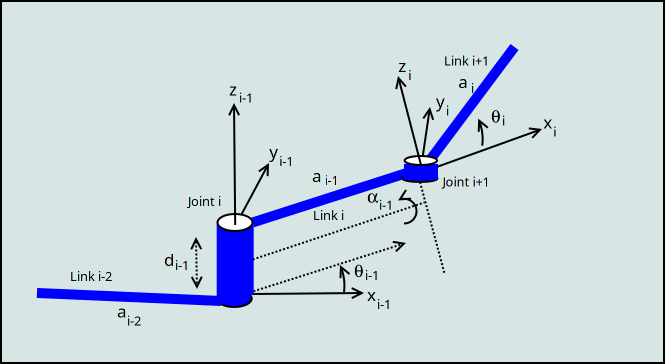
\includegraphics[width=0.5\textwidth,height=\textheight]{TermsFigures/DH.png}
\caption{}
\end{figure}

\begin{figure}
\centering
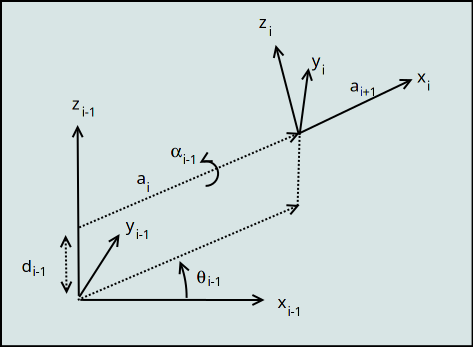
\includegraphics[width=0.6\textwidth,height=\textheight]{TermsFigures/DH2.png}
\caption{}
\end{figure}

Thus, the transformation from one joint to the next involves a rotation,
translation, translation and a rotation:

\begin{itemize}
\tightlist
\item
  Rotate about the local z axis angle \(\theta\).
\item
  Translate (offset) along the z axis amount \(d\).
\item
  Translate (link length) along x (common normal) amount \(a\).
\item
  Rotate about the x (common normal) axis (the joint twist) amount
  \(\alpha\).
\end{itemize}

This set of transformations will then change the coordinate system to
the next link in the serial chain.

\begin{figure}
\centering
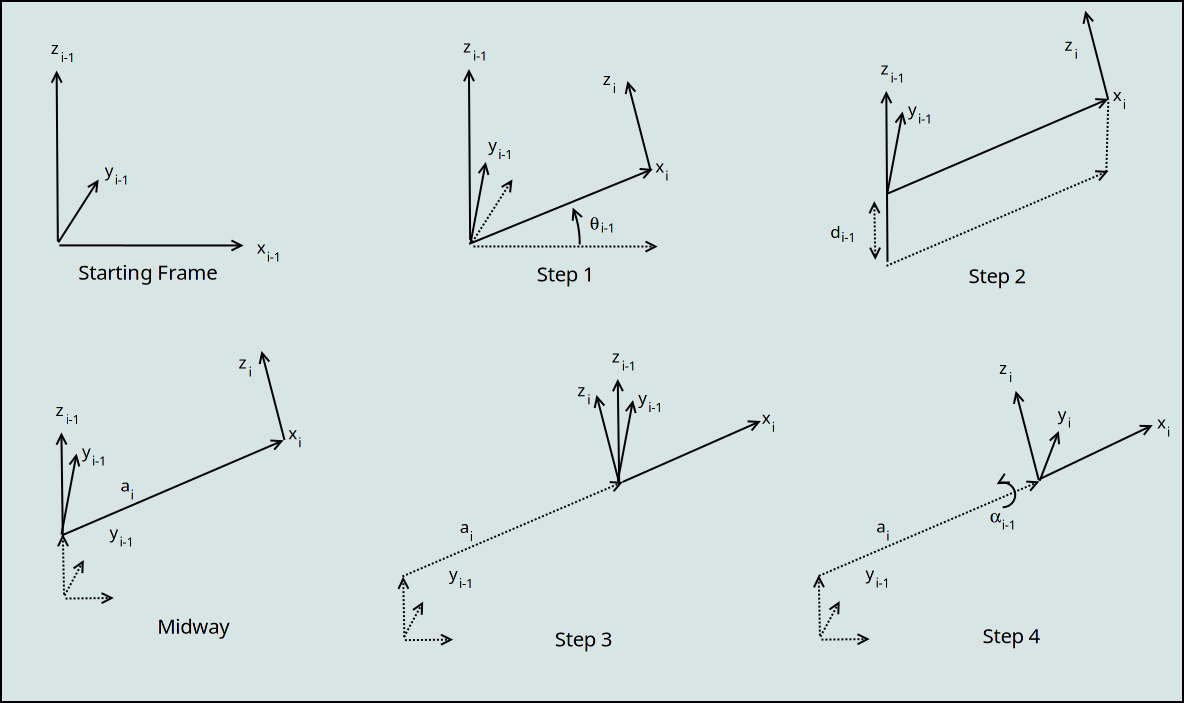
\includegraphics[width=0.75\textwidth,height=\textheight]{TermsFigures/DH3.png}
\caption{}
\end{figure}

\(A_{n} =\)

\[\begin{aligned}
\begin{pmatrix}\cos \theta_{n} & -\sin \theta_{n} & 0 & 0 \\
         \sin \theta_{n} & \cos \theta_{n} & 0 & 0\\ 0 &0 & 1 & 0 \\
         0& 0& 0& 1 \end{pmatrix}
         \begin{pmatrix}1 & 0 & 0 & 0 \\ 0 & 1 & 0 & 0  \\
         0& 0 & 1 & d_{n} \\
         0& 0& 0& 1 \end{pmatrix}
         \begin{pmatrix}1 & 0 & 0 & a_{n} \\ 0 & 1 & 0 & 0  \\
         0& 0 & 1 & 0 \\
         0& 0& 0& 1 \end{pmatrix}
\end{aligned}\]

\[\begin{aligned}
\times
 \begin{pmatrix}1 & 0 & 0 & 0 \\ 0 & \cos \alpha_{n} & -\sin \alpha_{n} & 0  \\
         0& \sin \alpha_{n} & \cos \alpha_{n} & 0 \\
         0& 0& 0& 1 \end{pmatrix}
\end{aligned}\]

\(A_{n} =\)

\[\begin{aligned}
\begin{pmatrix}\cos \theta_{n} & -\sin \theta_{n}\cos \alpha_{n} & \sin \theta_{n}\sin \alpha_{n} & a_{n}\cos \theta_{n} \\
\sin \theta_{n} & \cos \theta_{n}\cos \alpha_{n} & -\cos \theta_{n}\sin \alpha_{n}  & a_{n}\sin \theta_{n} \\ 0 & \sin \alpha_{n}& \cos \alpha_{n} & d_{n} \\
0& 0& 0& 1 \end{pmatrix}
\end{aligned}\]

A parameter table keeps track for each link, the values of \(\theta\),
\(d\), \(a\) and \(\alpha\).

Starting from the base of the robot, we can built the transformation
that defines the kinematics:

\[A = A_1A_2 \dots A_n = \prod_{i=1}^n A_i\]

Before we proceed with the examples, it is useful to summarize what has
been done. Using the DH notation, we can construct the transformation at
each joint. Taking the product of those transformations gives us the
relationship of the end-effector (tool tip) to the base coordinate
system or frame. The transformation is

\[\begin{aligned}
A =
\begin{pmatrix} a_{11}(q) & a_{12}(q) & a_{13}(q) & p_1(q) \\
a_{21}(q) & a_{22}(q) & a_{23}(q) & p_2(q) \\
a_{31}(q) & a_{32}(q) & a_{33}(q) & p_3(q) \\
0 & 0 & 0 & 1 \end{pmatrix} =
\begin{pmatrix} \vec{n} & \vec{o} & \vec{a} & \vec{p} \\ 0 & 0 & 0 & 1 \end{pmatrix}
\end{aligned}\]

The position of the end-effector can be extracted as
\(\vec{p} = <p_1, p_2, p_3>\) and the direction of the tip is given by
\(\vec{a}=<a_1,a_2,a_3>\). This is not the orientation vector and we
need to be careful here with orientation. What we mean is this is not
the orientation as a vector of Euler angles. Euler angles provide the
rotations about the axes (x, y, z) which would relate tool tip to the
x-axis in the base frame. The Euler angles orientation vector, \(\phi\)
can be difficult to find in general and often one does not have an
analytic representation. The value \(\phi\) is needed if one wanted to
computer the angular velocity of the tool tip.

\hypertarget{d-h-two-link-example}{%
\subsection{D-H Two Link Example}\label{d-h-two-link-example}}

\begin{longtable}[]{@{}lllll@{}}
\toprule
\begin{minipage}[b]{0.08\columnwidth}\raggedright
Link\strut
\end{minipage} & \begin{minipage}[b]{0.23\columnwidth}\raggedright
\(\theta\)\strut
\end{minipage} & \begin{minipage}[b]{0.14\columnwidth}\raggedright
\(d\)\strut
\end{minipage} & \begin{minipage}[b]{0.17\columnwidth}\raggedright
\(a\)\strut
\end{minipage} & \begin{minipage}[b]{0.20\columnwidth}\raggedright
\(\alpha\)\strut
\end{minipage}\tabularnewline
\midrule
\endhead
\begin{minipage}[t]{0.08\columnwidth}\raggedright
1\strut
\end{minipage} & \begin{minipage}[t]{0.23\columnwidth}\raggedright
\(\theta_1\)\strut
\end{minipage} & \begin{minipage}[t]{0.14\columnwidth}\raggedright
0\strut
\end{minipage} & \begin{minipage}[t]{0.17\columnwidth}\raggedright
\(a_1\)\strut
\end{minipage} & \begin{minipage}[t]{0.20\columnwidth}\raggedright
0\strut
\end{minipage}\tabularnewline
\begin{minipage}[t]{0.08\columnwidth}\raggedright
2\strut
\end{minipage} & \begin{minipage}[t]{0.23\columnwidth}\raggedright
\(\theta_2\)\strut
\end{minipage} & \begin{minipage}[t]{0.14\columnwidth}\raggedright
0\strut
\end{minipage} & \begin{minipage}[t]{0.17\columnwidth}\raggedright
\(a_2\)\strut
\end{minipage} & \begin{minipage}[t]{0.20\columnwidth}\raggedright
0\strut
\end{minipage}\tabularnewline
\bottomrule
\end{longtable}

\[\begin{aligned}
A_1 =\begin{pmatrix}\cos \theta_1 & -\sin \theta_1 & 0 & a_1 \cos \theta_1 \\
         \sin \theta_1 & \cos \theta_1 & 0 & a_1 \sin \theta_1
        \\ 0 &0 & 1 & 0 \\
         0& 0& 0& 1 \end{pmatrix}
\end{aligned}\]

\[\begin{aligned}
A_2 =\begin{pmatrix}\cos \theta_2 & -\sin \theta_2 & 0 & a_2 \cos \theta_2 \\
         \sin \theta_2 & \cos \theta_2 & 0 & a_2 \sin \theta_2 \\ 0 &0 & 1 & 0 \\
         0& 0& 0& 1 \end{pmatrix}
\end{aligned}\]

So,

\[\begin{aligned}
A = A_1A_2 =
  \begin{pmatrix}\cos (\theta_1+\theta_2) & -\sin (\theta_1+\theta_2) & 0 & a_2 \cos (\theta_1+\theta_2) + a_1 \cos \theta_1 \\
\sin (\theta_1 +\theta_2) & \cos (\theta_1 +\theta_2) & 0 & a_2 \sin (\theta_1 +\theta_2) + a_1\sin \theta_1\\
         0 &0 & 1 & 0 \\
         0& 0& 0& 1
  \end{pmatrix}
\end{aligned}\]

Then the location of the end effector \((x,y,z) = (p_x, p_y, p_z)\):

\[\begin{aligned}
\begin{pmatrix}
x \\ y \\ z
\end{pmatrix}
=
\begin{pmatrix}
a_2\cos (\theta_1+\theta_2) + a_1 \cos \theta_1 \\
a_2 \sin (\theta_1 +\theta_2) + a_1\sin \theta_1 \\
0
\end{pmatrix}
\end{aligned}\]

And it agrees with the earlier form.\footnote{Was there a great sigh of
  relief here? ... That the kinematic formulas for position agree with
  the ones found earlier.} As a planar function, we are not worried
about orientation around x or y. The \(\theta_i\) are all rotating
around a common direction, \(z\) . This implies that the orientation
about z is \(\phi = \theta_1 + \theta_2\).

\hypertarget{dh-inverse-kinematics}{%
\subsection{DH Inverse Kinematics}\label{dh-inverse-kinematics}}

It is much more difficult to find the inverse (parameters) functions if
you are given the end effector path:

\[p(t) \to \begin{pmatrix} \theta_1(t), ... , \theta_n(t)
           \end{pmatrix}\]

How can we use this technology to assist with the inverse kinematics
problem?

\[T^{-1}
  = T_0^{-1} T_{1}^{-1} \dots T_{n-1}^{-1} T_n^{-1}\]

In each matrix one can solve algebraically for \(\theta_i\) in terms of
the orientation and displacement vectors. What does this look like for
the two link manipulator?

Then we have that the transformation carries the frame to some frame
description \(A = F\):

\[\begin{aligned}
A = \begin{pmatrix}\cos (\theta_1+\theta_2) & -\sin (\theta_1+\theta_2) & 0 & a_2 \cos (\theta_1+\theta_2) + a_1 \cos \theta_1 \\
\sin (\theta_1 +\theta_2) & \cos (\theta_1 +\theta_2) & 0 & a_2 \sin (\theta_1 +\theta_2) + a_1\sin \theta_1\\
         0 &0 & 1 & 0 \\
         0& 0& 0& 1
  \end{pmatrix}
\end{aligned}\]

\[\begin{aligned}
=
  \begin{pmatrix}
         n_x & o_x & a_x & p_x \\
         n_y & o_y & a_y & p_y\\
         n_z & o_z & a_z & p_z \\
         0  &  0  &  0 & 1 \end{pmatrix} = F
\end{aligned}\]

Reversing the sequence of matrices does not give the inverse kinematics.
Going forward along the product of the matrices traces a path along the
robotic arm from the base to the tip given the joint angles. Reversing
the process takes us from the tip to the base given that set of joint
angles. What we want is a function that give the tip location, we
determine the various rotation angles. However, this reverse stacking of
the transformation matrices can help one in the algebraic process of
working out the inverse functions. In other words, it provides a
structure to do the function inverse. Recall the reverse ordering:

\[T^{-1}
  = T_0^{-1} T_{1}^{-1} \dots T_{n-1}^{-1} T_n^{-1}\]

In each matrix one can solve algebraically for \(\theta_i\) in terms of
the orientation and displacement vectors. What does this look like for
the two link manipulator?

Recall that

\[\begin{aligned}
A_1 =\begin{pmatrix}\cos \theta_1 & -\sin \theta_1 & 0 & a_1 \cos \theta_1 \\
         \sin \theta_1 & \cos \theta_1 & 0 & a_1 \sin \theta_1
        \\ 0 &0 & 1 & 0 \\
         0& 0& 0& 1 \end{pmatrix}
\end{aligned}\]

\[\begin{aligned}
A_2 =\begin{pmatrix}\cos \theta_2 & -\sin \theta_2 & 0 & a_2 \cos \theta_2 \\
         \sin \theta_2 & \cos \theta_2 & 0 & a_2 \sin \theta_2 \\ 0 &0 & 1 & 0 \\
         0& 0& 0& 1 \end{pmatrix}
\end{aligned}\]

Thus

\[\begin{aligned}
A = A_1(\theta_1)A_2(\theta_2) = \begin{pmatrix}
         n_x & o_x & a_x & p_x \\
         n_y & o_y & a_y & p_y\\
         n_z & o_z & a_z & p_z \\ 0 & 0 & 0 & 1\end{pmatrix}
\end{aligned}\]

Right multiply to decouple: \(A_1 = A A_2^{-1}\)

\[\begin{aligned}
=\begin{pmatrix}\cos \theta_1 & -\sin \theta_1 & 0 & a_1 \cos \theta_1 \\
         \sin \theta_1 & \cos \theta_1 & 0 & a_1 \sin \theta_1
        \\ 0 &0 & 1 & 0 \\
         0& 0& 0& 1 \end{pmatrix}
\end{aligned}\]

\[\begin{aligned}
= \begin{pmatrix}
         n_x & o_x & a_x & p_x \\
         n_y & o_y & a_y & p_y\\
         n_z & o_z & a_z & p_z \\ 0 & 0 & 0 & 1\end{pmatrix}
         \begin{pmatrix}\cos \theta_2 & -\sin \theta_2 & 0 & -a_2  \\
         \sin \theta_2 & \cos \theta_2 & 0 & 0 \\ 0 &0 & 1 & 0 \\
         0& 0& 0& 1 \end{pmatrix}
\end{aligned}\]

Note that \(a_1\cos\theta_1 = p_x - a_2n_x\) and
\(a_1\sin\theta_1 = p_y - a_2n_y\)

This provides us with

\[\theta_1 = \mbox{atan2}\left(\frac{p_y - a_2n_y}{a_1} , \frac{p_x - a_2n_x}{a_1}\right)\]

From \(\cos \theta_1 = \cos \theta_2 n_x - \sin \theta_2o_x\) and
\(-\sin \theta_1 = \sin \theta_2 n_x + \cos \theta_2o_x\)\\
we can solve for \(\theta_2\).

\[\begin{aligned}
\begin{pmatrix} \cos \theta_1 \\ -\sin \theta_1 \end{pmatrix}
  = \begin{pmatrix}n_x & -o_x  \\ n_x & o_x \end{pmatrix}
  \begin{pmatrix} \cos \theta_2 \\ \sin \theta_2 \end{pmatrix}
\end{aligned}\]

\[\begin{aligned}
\begin{pmatrix} \cos \theta_2 \\ \sin \theta_2 \end{pmatrix}
  = \frac{1}{2n_xo_x}\begin{pmatrix}o_x & o_x  \\ -n_x & n_x \end{pmatrix}
  \begin{pmatrix} \cos \theta_1 \\ -\sin \theta_1 \end{pmatrix}
\end{aligned}\]

So ...
\(\theta_2 = \mbox{atan2} \left( o_x(\cos \theta_1 -\sin \theta_1 ), -n_x(\cos \theta_1 +\sin \theta_1 )\right)\)

There is a problem. The two link example has two degrees of freedom. The
assumption here is that you have four variables to input (four degrees
of freedom): \(p_x, p_y, n_x, n_y\). You may not know
\(n_x, n_y\).\footnote{We will explore this more in the next section.}
For general systems this approach will succeed if you have enough
degrees of freedom in your robot.

\hypertarget{three-link-manipulator}{%
\subsection{\texorpdfstring{\texttt{Three\ link\ manipulator}}{Three link manipulator}}\label{three-link-manipulator}}

A simple extension of the two link is the three link planar manipulator.
It has DH parameters as

\begin{longtable}[]{@{}lllll@{}}
\toprule
\begin{minipage}[b]{0.08\columnwidth}\raggedright
Link\strut
\end{minipage} & \begin{minipage}[b]{0.23\columnwidth}\raggedright
\(\theta\)\strut
\end{minipage} & \begin{minipage}[b]{0.14\columnwidth}\raggedright
\(d\)\strut
\end{minipage} & \begin{minipage}[b]{0.17\columnwidth}\raggedright
\(a\)\strut
\end{minipage} & \begin{minipage}[b]{0.20\columnwidth}\raggedright
\(\alpha\)\strut
\end{minipage}\tabularnewline
\midrule
\endhead
\begin{minipage}[t]{0.08\columnwidth}\raggedright
1\strut
\end{minipage} & \begin{minipage}[t]{0.23\columnwidth}\raggedright
\(\theta_1\)\strut
\end{minipage} & \begin{minipage}[t]{0.14\columnwidth}\raggedright
0\strut
\end{minipage} & \begin{minipage}[t]{0.17\columnwidth}\raggedright
\(a_1\)\strut
\end{minipage} & \begin{minipage}[t]{0.20\columnwidth}\raggedright
0\strut
\end{minipage}\tabularnewline
\begin{minipage}[t]{0.08\columnwidth}\raggedright
2\strut
\end{minipage} & \begin{minipage}[t]{0.23\columnwidth}\raggedright
\(\theta_2\)\strut
\end{minipage} & \begin{minipage}[t]{0.14\columnwidth}\raggedright
0\strut
\end{minipage} & \begin{minipage}[t]{0.17\columnwidth}\raggedright
\(a_2\)\strut
\end{minipage} & \begin{minipage}[t]{0.20\columnwidth}\raggedright
0\strut
\end{minipage}\tabularnewline
\begin{minipage}[t]{0.08\columnwidth}\raggedright
3\strut
\end{minipage} & \begin{minipage}[t]{0.23\columnwidth}\raggedright
\(\theta_3\)\strut
\end{minipage} & \begin{minipage}[t]{0.14\columnwidth}\raggedright
0\strut
\end{minipage} & \begin{minipage}[t]{0.17\columnwidth}\raggedright
\(a_3\)\strut
\end{minipage} & \begin{minipage}[t]{0.20\columnwidth}\raggedright
0\strut
\end{minipage}\tabularnewline
\bottomrule
\end{longtable}

Products of the transformation matrices (and some trig) give us

\[\begin{aligned}
\begin{pmatrix}c_{123} & -s_{123} & 0 & a_3 c_{123} + a_2 c_{12} + a_1 c_1 \\
   s_{123} & c_{123} & 0 & a_3 s_{123} + a_2 s_{12} + a_1s_1\\
         0 &0 & 1 & 0 \\
         0& 0& 0& 1
\end{pmatrix}
\end{aligned}\]

where \(c_1 = \cos(\theta_1)\), \(c_{12} = \cos(\theta_1+\theta_2)\),
\(c_{123} = \cos(\theta_1+\theta_2+\theta_3)\),
\(s_1 = \sin(\theta_1)\), \(s_{12} = \sin(\theta_1+\theta_2)\),
\(s_{123} = \sin(\theta_1+\theta_2+\theta_3)\).

Extending the 2D result, the orientation (about z)
\(\phi = \theta_1+\theta_2+\theta_3\).

The IK formulas for the three link manipulator can be extrapolated from
the two link manipulator. The workspace for this manipulator is two
dimensional (x,y) and the configuration space is three dimensional
\((\theta_1, \theta_2, \theta_3 )\). We don't expect an inverse function
going from \({\Bbb R}^2 \to {\Bbb R}^3\). We expect on degree of freedom
on the inverse and intuitively we should be able to select location and
approach angle. So we an select \((x, y, \phi)\) with some restrictions
based on the workspace envelope.

The approach angle \(\phi = \theta_1 + \theta_2 + \theta_3\). Using the
approach angle \(\phi\) and the link length, we can find the joint
location of the joint 3:

\[W = (w_x, w_y) = (x - a_3\cos\phi , y - a_3\sin\phi)\]

Backing up to \(W\) means we can employ the two link formulas.

\[c_2 = \frac{w_x^2 + w_y^2 - a_1^2 - a_2^2}{2a_1a_2} , \quad s_2  = \pm \sqrt{1 - c_2^2}, \quad
\theta_2 = \mbox{atan2}(s_2,c_2)\]

\[s_1 = \frac{(a_1+a_2)w_y - a_2s_2w_x}{w_x^2+w_y^2}, \quad c_1 = \frac{(a_1+a_2)w_x + a_2s_2w_y}{w_x^2+w_y^2}, \quad
\theta_1 = \mbox{atan2}(s_1, c_1), \quad \theta_3 = \phi - \theta_1 - \theta_2\]

This gives one degree of freedom parameterized by \(\phi\) {[}if you see
this as a function of (x,y){]}.

\hypertarget{numerica-inverse-kinematics-1}{%
\subsection{Inverse kinematics numerical
approaches}\label{numerica-inverse-kinematics-1}}

A number of robotics engineers will tell you that you want to design
your robot with inverse kinematics in mind. This means keeping the
design simple when possible, having ways to partition the system so that
components can be controlled separately and leverage existing design
when it makes sense. If you do need to know joint values as a function
of position, this can be approximated numerically. The FK equations can
be intimidating, but they are nonlinear algebraic equations. There are
approaches to solving systems of nonlinear equations. The tools fall in
gradient based and gradient free approaches. The gradient methods, as
the name implies, require derivatives to be supplied to the solver.
Gradient free methods do not. We will look at numerical methods in the
simulation chapter and leave off here with the comment that in many
cases we can find good numerical inverses even when we cannnot do so
analytically.
